\section{Hypergraph-based Methods for Clustering and Classification}
%%%%%%%%%%%%%%%%%%%%%%%%%%%%%%%%%%%%%%%%%%%%%%%%%%%%%%%%%%%%%%%%%%%%%%%%%%%%%%%%%%%%%%%%%%%%%%%%%%%%%%%%%%%%%

\textbf{Classification}:
In classification, the goal is to find the correct labels for the unlabeled instances given a finite set of labeled instances. In Figure~\ref{fig:bipartitegraph-weighted}, the leftmost partition corresponds to rows in the underlying relational table. Suppose a subset of vertices are labeled (e.g., $r_1$ is labeled $l_1$ and $r_4$ is labeled $l_2$), then the classification problem can be formulated as to discover correct labels for unlabeled vertices (e.g., $r_1$ and $r_3$). Conceptually, the pair of nodes being ``close to'' one another shall share the same labels, which are consistent to one basic principle of  semi-supervised learning. However, the challenge is how can we define the closeness between two nodes. We can still rely on the paths linking them where the path length becomes an important measure as well as the node labels.

\textbf{Clustering:}
Cluster analysis or clustering is the task of assigning a set of objects into groups (called clusters) so that the objects in the same cluster are more similar to each other than to those in other clusters. It is easy to observe that in Figure~\ref{fig:bipartitegraph-weighted}  the clustering of rows of the underlying relational table can be viewed as a neighborhood formation for vertices on the leftmost partition. Basically, for any closely related nodes, we should group them together. Especially, if we can derive an explicit  similarity/distance measure, then classical distance-based clustering algorithms, such as k-means, can be directly applied to cluster the vertices.

\subsection{Clustering Analysis}
\subsubsection{Distance-based Clustering}

\begin{figure}[tbh]
\centering
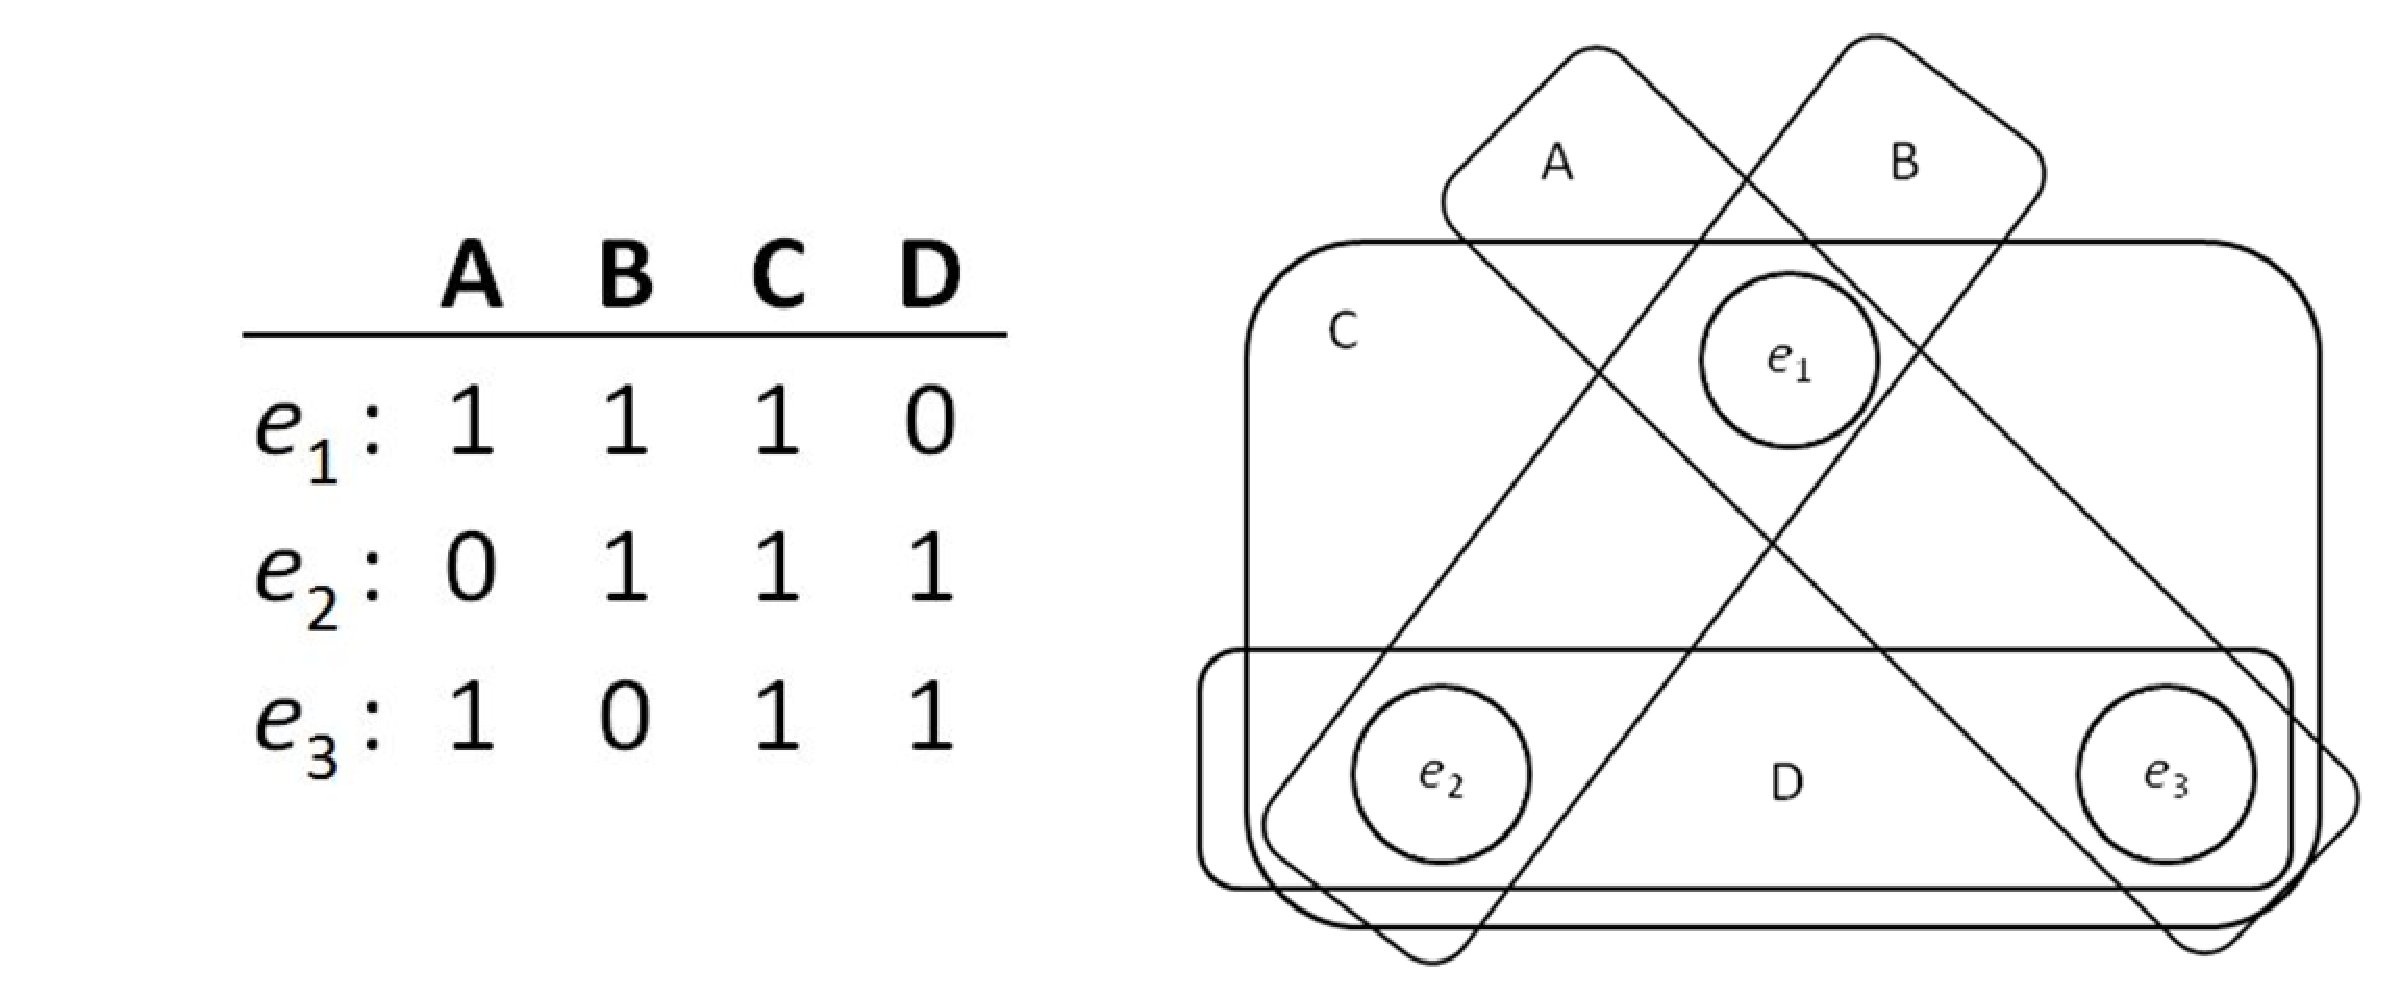
\includegraphics[width=.6\textwidth]{fig/hypergraph-column-wise.eps}
\caption{\label{fig:hypergraph-column-wise} .}
\end{figure}
Given the hypergraph-based technique for mining semantically associated itemsets presented in the last section, we can apply a ``turn around" of the perspective in the hypergraph model and extend it to cluster analysis. In Figure.~\ref{fig:hypergraph-column-wise} we show the same motivating example as that is used in mining semantically associated itemsets. Instead of creating a hyperedge for each row, we create one for each column. A row node is incident on the corresponding hyperedge if it has a value `1' in that column.

\subsubsection{Partition-based Clustering}
Given a set of data points $x_1, \ldots x_n$ and some notion of similarity $s(i,j) > 0$ between all pairs of data points $x_i$ and $x_j$ , the common definition of clustering is to divide the data points into several groups such that points in the same group are similar to each other than ones taken from other groups. The relationships among $n$ data points can be specified by means of an $n \times n$ similarity matrix, whose elements $s_{ij}$ measure the similarity of data points $x_i$ and $x_j$.

Partitional clustering algorithms obtain a single partition of the data that optimizes a certain criterion. The most widely used criterion is minimizing the overall squared distance between each data point and the center of its related cluster.

\begin{equation}
argmax_s\sum^k_{i=1}\sum_{x_j\in S}s(j,u_i)^2~, \label{eq:kmeans}
\end{equation}

where $u_i$ is the mean of points in $S_i$. If we restrict the centroids to members of the data, i.e., $u_i \in S_i$, the resulting clustering algorithm is called $k$-medoids algorithm. The optimization problem in Equation~\ref{eq:kmeans} itself is known to be NP-hard, and thus the common approach is to search only for approximate solutions. A particularly well known approximative method is Lloyd's algorithm~\cite{Lloyd83}.

There are several graph-based similarity measures that can be used in the partitional clustering algorithms. The shortest path distance on a graph (also known as the geodesic distance) can be used as the most straight forward measure.
The hypergraph commute time similarity introduced in Section~\ref{sec:assoc_noonto} is more appealing to be used for clustering purposes, because as opposed to the shortest path distance, the commute distance between two vertices decreases if there are many different short ways to get from vertex $v_i$ to vertex $v_j$ . So instead of just looking for the one shortest path, the commute distance looks at the set of short paths. Points which are connected by a short path in the graph and lie in the same high-density region of the graph are considered closer to each other than points which are connected by a short path but lie in different high-density regions of the graph.

\subsubsection{Spectral Clustering}
If we do not have more information than similarities between data points, a nice way of representing the data is in form of the similarity graph $G = (V,E)$. Each vertex vi in this graph represents a data point $x_i$. Two vertices are connected if the similarity $s_{ij}$ between the corresponding data points $x_i$ and $x_j$ is positive or larger than a certain threshold, and the edge is weighted by $s_{ij}$. The problem of clustering can now be reformulated using the similarity graph: we want to find a partition of the graph such that the edges between different groups have very low weights (which means that points in different clusters are dissimilar from each other) and the edges within a group have high weights (which means that points within the same cluster are similar to each other). To be able to formalize this intuition we first want to introduce some basic graph notation and briefly discuss the kind of graphs we are going to study.

The $\epsilon$-neighborhood graph: Here we connect all points whose pairwise distances are smaller than $\epsilon$. As the distances between all connected points are roughly of the same scale (at most $\epsilon$), weighting the edges would not incorporate more information about the data to the graph. Hence, the $\epsilon$-neighborhood graph is usually considered as an unweighted graph.

$k$-nearest neighbor graphs: Here the goal is to connect vertex $v_i$ with vertex $v_j$ if $v_j$ is among the $k$-nearest neighbors of $v_i$. However, this definition leads to a directed graph, as the neighborhood relationship is not symmetric. There are two ways of making this graph undirected. The first way is to simply ignore the directions of the edges, that is we connect $v_i$ and $v_j$ with an undirected edge if $v_i$ is among the k-nearest neighbors of $v_j$ or if $v_j$ is among the $k$-nearest neighbors of vi. The resulting graph is what is usually called the k-nearest neighbor graph. The second choice is to connect vertices $v_i$ and $v_j$ if both $v_i$ is among the k-nearest neighbors of $v_j$ and $v_j$ is among the $k$-nearest neighbors of $v_i$. The resulting graph is called the mutual $k$-nearest neighbor graph. In both cases, after connecting the appropriate vertices we weight the edges by the similarity of their endpoints.

The fully connected graph: Here we simply connect all points with positive similarity with each other, and we weight all edges by $s_{ij}$ . As the graph should represent the local neighborhood relationships, this construction is only useful if the similarity function itself models local neighborhoods. An example for such a similarity function is the Gaussian similarity function $s(x_i, x_j) = e^{-\|x_i - x_j\|^2/(2\sigma^2)}$, where the parameter $\sigma$ controls the width of the neighborhoods. This parameter plays a similar role as the parameter $\epsilon$ in case of the $\epsilon$-neighborhood graph.


%%%%%%%%%%%%%%%%%%%%%%%%%%%%%%%%%%%%%%%%%%%%%%%%%%%%%%%%%%%%%%%%%%%%%%%%%%%%%%%%%%%%%%%%%%%%%%%%%%%%%%%%%%%%%
\subsection{Classification}
\label{sec:classification}
The hypergraph representation for the problem of classification is similar to the one for clustering. We can create hyperedges for columns in the same way as shown in Figure~\ref{fig:hypergraph-column-wise} with the only difference being that a portion of row nodes is labeled and rest unlabeled. The goal for classification is to utilize the information in labeled nodes to come up with correct labels for unlabeled ones.

This problem can be solved by hypergraph-based label propagation. Let $f$ be the objective function (vector) of labels to be learned. Intuitively, there are two criteria for learning the optimal $f$ : (1) we want to assign the same label to vertices that share many incidental hyperedges in common; and (2) assignment of the labels should be similar to the initial labeling $y$. For criteria (1), we define the following cost function
\begin{equation}
\Omega(f,w)=\frac{1}{2}\sum_{e\in E}\sum_{u,v\in e}\frac{w(e)h(u,e)h(v,e)}{d(e)} ~.
\end{equation}
where $I$ is the identity matrix. Here, $D_v$ and $D_e$ are used for computing the normalization of the hypergraph Laplacian, and the unnormalized hypergraph Laplacian is $diag(HD_ew)HWH^T$ . Empirical results showed that the normalized form gives better classification performance for graphbased learning~\cite{Zhou2006}. If the predicted labels on the vertices are consistent with the incidences with the hyperedges, the value of $\Omega(f,w)$ should be minimized. For criteria (2), we directly calculate the squared-loss between the predicted labeling f and the original labeling y as follows,
\begin{equation}
\notag \sum_{u\in V}(f(u)-y(u))^2=\|f-y\|^2
\end{equation}
%%%%%%%%%%%%%%%%%%%%%%%%%%%%%%%%%%%%%%%%%%%%%%%%%%%%%%%%%%%%%%%%%%%%%%%%%%%%%%%%%%%%%%%%%%%%%%%%%%%%%%%%%%%%%